\subsection{Eixos Temáticos de Conteúdo}

\begin{figure}[!htbp]
\centering
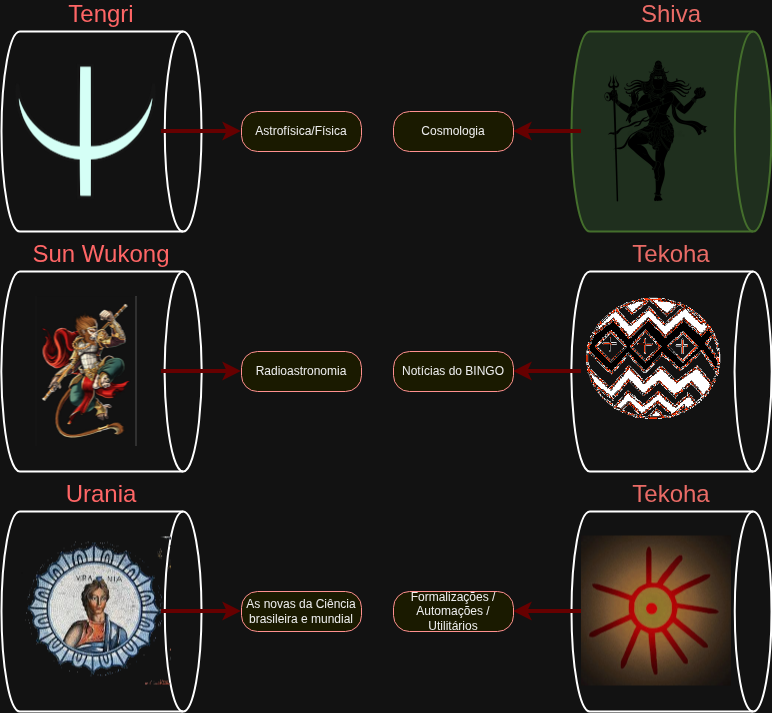
\includegraphics[width=1\linewidth]{files/eixos-dab8b38ab807d2296e5902c857fb6f08.png}
\end{figure}

\subsubsection{Conteúdos por Eixo}

\begin{itemize}
\item \textbf{Tengre:}

\begin{itemize}
\item Como medimos distâncias em astronomia,
\item Evolução de estrelas,
\item Pulsares,
\item Fenômenos transientes de Rádio,
\item Pulsar Timing Array,
\item Ondas Gravitacionais
\end{itemize}


\item \textbf{Shiva Nataraja:}

\begin{itemize}
\item A história térmica do universo,
\item Desacoplamento e recombinação,
\item Composição do Universo,
\item Matéria escura,
\item Energia escura,
\item Tensão de Hubble
\end{itemize}


\item \textbf{Sun Wukong:}

\begin{itemize}
\item Espectro eletromagnético,
\item Antenas e receptores,
\item Sinais digitais de rádio,
\item Interferências eletromagnéticas,
\item Planejamento de observações,
\item Espectrômetro,
\item Hidrogênio neutro
\end{itemize}


\item \textbf{Tekoha:}

\begin{itemize}
\item Editais e calendário,
\item Publicações,
\item Premiações,
\item Agenda de Eventos,
\item Modelos digitais,
\item Andamento da construção,
\item Notícias das Universidades,
\item Bolsistas
\end{itemize}


\item \textbf{Urania:}

\begin{itemize}
\item Notícias internacionais,
\item Clipping de ciência,
\item Featured article of the month
\end{itemize}


\item \textbf{Guaraci:}

\begin{itemize}
\item Portal,
\item Templates,
\item Workflows,
\item Automação,
\item Relatórios,
\item Press releases,
\item Apresentações para financiadores
\end{itemize}
\end{itemize}


\bigskip
\centerline{\rule{13cm}{0.4pt}}
\bigskip